\chapter{混合、振盪、電偶極矩與場算符}

我們先從一個稍微偏離本章主題的問題談起：中微子。有證據顯示中微子具有質量，而且不同種類的中微子會發生混合。如果它們的質量並不全都相同，為什麼一種中微子可以轉變成另一種，卻不違反能量守恆？

這個問題帶出量子力學中反覆出現的一種結構：製備或測量系統時所對應的態，不一定是讓哈密頓量對角化的態。確定能量的態只會獲得相位；若製備的態是數個能量本徵態的疊加，各分量因獲得不同相位，整個態便會改變。這個區別將帶我們從雙勢阱談到中微子振盪與自旋進動。接著我們會插談電子電偶極矩，再回到二次量子化，看看同樣的位置--動量傅立葉結構如何出現在算符層次。

\section{問題的核心是混合}

中微子的質量不必全都相同。能量本徵態彼此不會混合；每個本徵態都獨立演化。我們所說的中微子\emph{種類}，也就是味，與中微子的產生和測量方式有關；味態則可以是質量能量本徵態的線性組合。概略地說，
\begin{equation}
|\text{type}\rangle = \sum_n c_n |E_n\rangle .
\end{equation}
因此，正確的說法不是能量本徵態彼此轉變，而是稱為``電子中微子''或``{\proseunicodefont μ}子中微子''的態，本身不一定是能量本徵態。

\begin{classroomqa}
\lecturetimestamp{00:00:09}
\audiencequestion{如果中微子具有不同質量，它們如何能在能量守恆的情況下混合？}
\lecturerresponse{質量能量本徵態不會彼此轉變。電子味、{\proseunicodefont μ}子味和{\proseunicodefont τ}味態，是這些本徵態的不同線性組合。各質量分量分別依自己的相位演化；分量間的干涉會改變各味的機率，但不違反能量守恆。}
\end{classroomqa}

這種結構有許多例子。最直觀的一個例子，是粒子處於對稱雙勢阱中。

\section{對稱雙勢阱與近似定域態}

考慮一個粒子在對稱雙勢阱中運動，兩個勢阱最低點之間隔著一道高勢壘。若勢壘無限高，左右兩個勢阱便會完全解耦。我們可以把右側視為不存在，只求解左側勢阱；右側也可以同樣處理。近似的基態波函數便是左側定域態\(\psi_L\)與右側定域態\(\psi_R\)，兩者的能量相同\(E\)。

在每個孤立的勢阱中，基態都有熟悉的定性特徵：波函數平滑、沒有節點，並且處於符合束縛條件的最低能量。可以把中央的高勢壘想成一道磚牆。把它視為無限高只是近似，但能讓我們先從一對有用的定域態開始。

\begin{figure}
\centering
\begin{adjustbox}{max width=\linewidth}
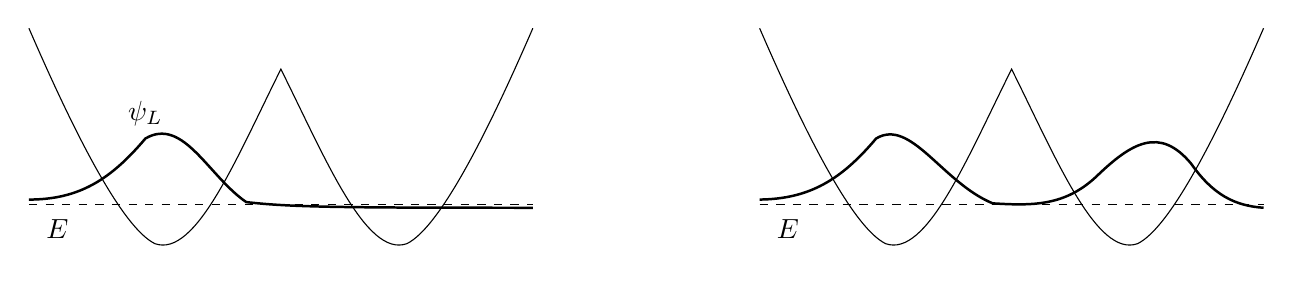
\begin{tikzpicture}[x=0.8cm,y=0.8cm]
\begin{scope}[shift={(-5.8,0)}]
\draw (-4,2.7) .. controls (-3.35,1.2) and (-2.55,-0.45) .. (-2.0,-0.72)
      .. controls (-1.35,-0.95) and (-0.7,0.65) .. (0,2.05)
      .. controls (0.7,0.65) and (1.35,-0.95) .. (2.0,-0.72)
      .. controls (2.55,-0.45) and (3.35,1.2) .. (4,2.7);
\draw[dashed] (-4,-0.10) -- (4,-0.10);
\node at (-3.55,-0.48) {$E$};
\draw[line width=0.9pt] (-4,-0.02) .. controls (-3.2,-0.02) and (-2.7,0.30) .. (-2.15,0.95)
      .. controls (-1.55,1.30) and (-1.15,0.35) .. (-0.55,-0.06)
      .. controls (0.15,-0.14) and (0.9,-0.15) .. (4,-0.15);
\node at (-2.15,1.35) {$\psi_L$};
\end{scope}
\begin{scope}[shift={(5.8,0)}]
\draw (-4,2.7) .. controls (-3.35,1.2) and (-2.55,-0.45) .. (-2.0,-0.72)
      .. controls (-1.35,-0.95) and (-0.7,0.65) .. (0,2.05)
      .. controls (0.7,0.65) and (1.35,-0.95) .. (2.0,-0.72)
      .. controls (2.55,-0.45) and (3.35,1.2) .. (4,2.7);
\draw[dashed] (-4,-0.10) -- (4,-0.10);
\node at (-3.55,-0.48) {$E$};
\draw[line width=0.9pt] (-4,-0.02) .. controls (-3.2,-0.01) and (-2.7,0.30) .. (-2.15,0.95)
      .. controls (-1.6,1.28) and (-1.1,0.25) .. (-0.30,-0.08)
      .. controls (0.35,-0.12) and (0.85,-0.12) .. (1.35,0.35)
      .. controls (1.9,0.88) and (2.35,1.15) .. (2.85,0.55)
      .. controls (3.2,0.05) and (3.55,-0.12) .. (4,-0.15);
\end{scope}
\end{tikzpicture}
\end{adjustbox}
\caption{開場板書草圖的清晰重繪。左圖是單側試探態\(\psi_L\)，是把勢壘視為實際上無限高時得到的結果。右圖則將同一波函數對稱地延伸至勢壘另一側，顯示波函數有少量但非零的穿透，最終形成真正的偶宇稱基態。}
\end{figure}

然而，在量子力學中，勢壘並非真正無限高。勢壘區域中的波函數不會恰好等於零，只是非常小。這一點微弱的穿透正是關鍵所在；它使左右兩側的近似描述成為真正的混合問題。

\section{宇稱本徵態與指數級能階分裂}

現在，定域態的圖像要讓位給一個定理：若位勢具有對稱性，精確的能量本徵函數就可以選成在反射下為對稱態或反對稱態。

\begin{theorem}
若一維位勢滿足\(V(x)=V(-x)\)，則哈密頓量的本徵函數可以選成滿足以下其中一種關係：
\[
\psi(x)=\psi(-x)
\qquad \text{or} \qquad
\psi(x)=-\psi(-x).
\]
\end{theorem}

接著要修正先前的近似。單側態\(\psi_L\)與\(\psi_R\)既不對稱，也不反對稱，因此不可能是完整哈密頓量的精確本徵態。只有在勢壘很高時，它們才是良好的近似態。真正的本徵態是對稱與反對稱的線性組合：
\begin{align}
\psi_+ &= \frac{\psi_L+\psi_R}{\sqrt{2}},\\
\psi_- &= \frac{\psi_L-\psi_R}{\sqrt{2}}.
\end{align}
沿用留在黑板上的記號，將它們的能量標為
\begin{align}
H\psi_+ &= (E_1-\epsilon)\psi_+,\\
H\psi_- &= (E_1+\epsilon)\psi_-.
\end{align}
因此，兩能階的總分裂為
\begin{equation}
\Delta E = (E_1+\epsilon)-(E_1-\epsilon)=2\epsilon .
\end{equation}

\begin{figure}[htbp]
\centering
\includegraphics[width=0.92\linewidth]{lecture_08_frame_02.png}
\caption{雙勢阱中的對稱延伸波函數。波函數在勢壘下方的振幅雖小但不為零，能階分裂正是由此而來。}
\lectureframe{00:06:19}
\end{figure}

\begin{figure}
\centering
\begin{tikzpicture}[x=1cm,y=1cm]
\draw[->] (0,0) -- (0,3);
\node[left] at (0,2.8) {energy};
\draw (-0.35,1.60) -- (0.35,1.60);
\node[left] at (-0.45,1.60) {$\psi_L,\psi_R$};
\node at (1.7,1.60) {$\Longrightarrow$};
\draw (3.0,1.32) -- (3.75,1.32);
\draw (3.0,1.88) -- (3.75,1.88);
\draw[dashed] (2.8,1.60) -- (3.95,1.60);
\node[right] at (3.9,1.32) {$\psi_+,\ E_1-\epsilon$};
\node[right] at (3.9,1.88) {$\psi_-,\ E_1+\epsilon$};
\node[below] at (3.37,1.60) {$E_1$};
\end{tikzpicture}
\caption{隧穿分裂的板書推導。近似的左側態與右側態幾乎簡併，但精確的對稱與反對稱本徵態之間仍有微小能量差\(2\epsilon\)。}
\end{figure}

能階的高低順序反映了其中的物理。對稱態的能量稍低，因為它在勢壘區域較平滑；波函數得以穿透勢壘並對稱延伸，會使能量降低一點點。反對稱態的能量稍高，因為一維系統的第一激發態有一個節點，而在這個對稱問題中，節點位於中點。額外的曲率會增加動能。

這個效應非常小，而且隨勢壘的寬度與高度呈指數級變小。這裡不需要寫出明確的 WKB 公式；重要的是，能階分裂確實存在，只是非常微小。另外要記得，波函數的整體正負號不具物理意義。將\(\psi_-\)換成\(-\psi_-\)，不會改變這個態。

\section{時間演化與左右振盪}

現在來問動力學問題：若一開始把粒子置於左側勢阱，會發生什麼事？這是關鍵的一步，因為振盪正是同一混合現象在時間演化中的呈現。

反向關係為
\begin{align}
\psi_L &= \frac{\psi_+ + \psi_-}{\sqrt{2}},\\
\psi_R &= \frac{\psi_+ - \psi_-}{\sqrt{2}}.
\end{align}
因此，初始時局域在左側的態是
\begin{equation}
\psi(0)=\psi_L=\frac{\psi_+ + \psi_-}{\sqrt{2}}.
\end{equation}
它不是能量本徵態，所以必然會發生非平凡的時間演化。

我們採用標準的Schr\"odinger約定\(e^{-iEt}\)。共同相位不會造成可觀測效應；只有兩個能量分量之間的相對相位，才能使機率從一個勢阱轉移到另一個勢阱。

依照這個約定，
\begin{equation}
\psi(t)=\frac{1}{\sqrt{2}}\left(e^{-i(E_1-\epsilon)t}\psi_+ + e^{-i(E_1+\epsilon)t}\psi_-\right).
\end{equation}
這是整理後的板書公式。現在提出共同相位：
\begin{equation}
\psi(t)=\frac{e^{-iE_1 t}}{\sqrt{2}}\left(e^{i\epsilon t}\psi_+ + e^{-i\epsilon t}\psi_-\right).
\end{equation}
此時，一個相位沿單位圓朝一個方向變化，另一個則朝相反方向變化。態之所以改變，只是因為兩個相位逐漸不同步。

將\(\psi_\pm\)的定義代入，就能明確看出左右振盪：
\begin{align}
\psi(t)
&= \frac{e^{-iE_1 t}}{2}
\left[e^{i\epsilon t}(\psi_L+\psi_R)+e^{-i\epsilon t}(\psi_L-\psi_R)\right] \\
&= \frac{e^{-iE_1 t}}{2}
\left[(e^{i\epsilon t}+e^{-i\epsilon t})\psi_L+(e^{i\epsilon t}-e^{-i\epsilon t})\psi_R\right] \\
&= e^{-iE_1 t}\left[\psi_L\cos(\epsilon t)+i\,\psi_R\sin(\epsilon t)\right].
\end{align}
這是本章的關鍵推導。在雙態近似下，若\(\psi_L\)與\(\psi_R\)正交歸一，兩側的機率為
\begin{equation}
P_L(t)=\cos^2(\epsilon t),
\qquad
P_R(t)=\sin^2(\epsilon t).
\end{equation}
因此，系統會振盪。在兩端之間的時刻，系統確實處於疊加態；例如，當\(\epsilon t=\pi/4\)時，粒子在兩側的機率相等。相位連續演化，定域程度也隨之連續改變。

黑板上的推導找出相對符號第一次反轉的時刻，也就是滿足下式的時刻：
\begin{equation}
e^{-i\epsilon t}=-\,e^{i\epsilon t},
\end{equation}
這是板書中清楚標出的關鍵條件。兩邊同乘後得到
\begin{equation}
e^{2i\epsilon t}=-1.
\end{equation}
第一次出現這種情況時，
\begin{equation}
2\epsilon t=\pi,
\qquad\text{so}\qquad
t_{L\to R}=\frac{\pi}{2\epsilon}.
\end{equation}

\begin{figure}[htbp]
\centering
\includegraphics[width=0.94\linewidth]{lecture_08_frame_05.png}
\caption{黑板上的相對相位計算。當\(e^{2i\epsilon t}=-1\)時，兩個能量分量的相位相差{\proseunicodefont π}，得到第一次轉移所需時間\(2\epsilon t=\pi\)。排版後的推導一致採用Schr\"odinger相位約定。}
\lectureframe{00:17:52}
\end{figure}
在這個時刻，
\begin{equation}
\psi(t_{L\to R}) \propto \frac{\psi_+-\psi_-}{\sqrt{2}}=\psi_R.
\end{equation}
整體相位無關緊要。重要的是，起初置於左側的粒子已演化成右側定域態。再經過同樣長的時間，它便會擺回左側。混合與振盪相伴而生。

方程所表示的結果很明確：\(\epsilon\)越小，振盪越慢，轉移所需時間越長。兩個定域態都沒有確定的能量；但兩個精確的能量分量各自守恆能量，並依照應有的方式演化。

\section{中微子、氨分子與自旋的類比}

雙勢阱提供了一個理解中微子問題的範例。與電子一同產生的中微子稱為電子中微子；與{\proseunicodefont μ}子一同產生的則稱為{\proseunicodefont μ}子中微子。這些味標籤描述產生與測量的通道。具有確定質量的態構成另一組基底；在動量固定時，它們也具有確定的自由粒子能量。

在最簡單的雙態最大混合示意模型中，
\begin{equation}
|\nu_e\rangle \sim \frac{|m_1\rangle+|m_2\rangle}{\sqrt{2}},
\qquad
|\nu_\mu\rangle \sim \frac{|m_1\rangle-|m_2\rangle}{\sqrt{2}},
\end{equation}
其中，質量本徵態對應\(\psi_+\)與\(\psi_-\)，味態則對應\(\psi_L\)與\(\psi_R\)。真實的中微子混合由非平凡的混合矩陣描述，係數並不相等；不過，這裡已能看出其作用機制。

電子中微子是在涉及電子的過程中產生的，就像粒子一開始被置於左側勢阱。在短距離傳播後，它的兩個質量分量所累積的相位幾乎相同，因此仍會在交互作用中被辨識為電子味。經過長距離傳播後，兩個相位便會分開。之後的帶電流交互作用可能產生{\proseunicodefont μ}子而非電子，表示該態已含有{\proseunicodefont μ}子味分量。在不同距離或能量下重複實驗，就能觀察到振盪。

這並不違反能量守恆。質量能量本徵態完全依照本徵態應有的方式演化；隨時間改變的是味疊加態。在相對論極限下，可觀測的相對相位取決於質量平方差，概略地說：
\begin{equation}
\Delta\phi_{ij}\simeq \frac{\Delta m_{ij}^{,2}L}{2E}.
\end{equation}
因此，觀察到振盪表示中微子的質量不可能全都相同；至少有兩個質量本徵態的質量不同。

\begin{classroomqa}
\lecturetimestamp{00:24:06}
\audiencequestion{雙勢阱例子中的微小能階分裂\(\epsilon\)由什麼決定？}
\lecturerresponse{它取決於粒子質量，以及勢壘的高度與寬度。隧穿對這些細節呈指數敏感，因此勢壘稍有變化，就可能使\(\epsilon\)的相對大小大幅改變。}
\end{classroomqa}

\begin{classroomqa}
\lecturetimestamp{00:24:26}
\audiencequestion{這種振盪現象真的觀測到了嗎？}
\lecturerresponse{是的。一般量子系統中觀測得到隧穿造成的能階分裂，中微子則有味振盪。兩者的微觀機制不同，但都呈現相同的雙態相位演化。}
\end{classroomqa}

\begin{classroomqa}
\lecturetimestamp{00:24:34}
\audiencequestion{中微子振盪與中微子質量有什麼關聯？}
\lecturerresponse{傳播中的本徵態具有不同質量，因此累積的相位也不同。這些分量彼此干涉，改變了味的組成。在符合實際情況的相對論描述中，控制振盪的是質量平方差，而不是單一粒子的質量真的隨時間變化。}
\end{classroomqa}

\begin{classroomqa}
\lecturetimestamp{00:25:02}
\audiencequestion{中微子質量只是主流理論的說法，還是實驗事實？}
\lecturerresponse{振盪是實驗事實，而且要求質量差不為零。絕對質量尺度是另一個更難測量的問題，但「所有中微子都沒有質量」這個最簡單的圖像已被實驗排除。}
\end{classroomqa}

\subsection{氨分子反轉：真實的勢壘}

氨分子\(\mathrm{NH}_3\)呈三角錐形：三個氫原子位於同一平面，氮原子則位於平面一側。氮原子位於另一側時，也有一個等價構型。這兩個定域構型都不是精確的定態。氮原子可以隧穿穿過氫原子所在的平面，形成對稱與反對稱的能量本徵態，並造成微小的反轉能階分裂。氨微波激射器中的相關數學結構，物理上正是源自這個效應。

\begin{classroomqa}
\lecturetimestamp{00:25:11}
\audiencequestion{在氨分子中，勢壘是否就是氮原子穿過氫原子所在平面時的構型？}
\lecturerresponse{是。分子在兩種三角錐構型下的能量都最低，平面構型的能量則較高。氮原子隧穿經過這個構型，便會耦合兩側。}
\end{classroomqa}

\begin{classroomqa}
\lecturetimestamp{00:27:10}
\audiencequestion{電子中微子與{\proseunicodefont μ}子中微子之間，對應的實際勢壘是什麼？}
\lecturerresponse{這裡沒有字面上的空間勢壘。這個類比只在代數結構上成立：中微子哈密頓量中的非對角耦合會使味基底發生混合。在氨分子中，這種耦合來自隧穿；對中微子而言，它是質量與混合結構的一部分。}
\end{classroomqa}

\subsection{自旋進動：不經由隧穿的混合}

我們已在自旋問題中見過相同的代數結構。考慮兩個態\(|\uparrow_z\rangle\)與\(|\downarrow_z\rangle\)。沒有磁場時，兩者能量簡併。現在施加沿\(x\)方向的磁場。能量本徵態不再是\(z\)本徵態，而是沿\(x\)方向偏極的態。沿用黑板上暫時採用的左--右標記，
\begin{align}
|L_x\rangle &= \frac{|\uparrow_z\rangle+|\downarrow_z\rangle}{\sqrt{2}},\\
|R_x\rangle &= \frac{|\uparrow_z\rangle-|\downarrow_z\rangle}{\sqrt{2}}.
\end{align}
這兩個態分別直接類比於\(\psi_+\)與\(\psi_-\)。磁矩沿磁場方向與反磁場方向排列時，能量略有差異。若能量為\(E\mp\epsilon\)，則初始朝上的自旋會演化為
\begin{equation}
|\uparrow_z,t\rangle
= e^{-iEt}\left[\cos(\epsilon t)\,|\uparrow_z\rangle
+ i\sin(\epsilon t)\,|\downarrow_z\rangle\right].
\end{equation}
這與雙勢阱的公式相同，只是此處的連續演化是自旋繞\(x\)軸進動。從\(+z\)出發，自旋會經過橫向取向，在半個進動週期後到達\(-z\)，再經過半個週期回到原處。測量\(S_z\)仍只會得到向上或向下；自旋態連續的變化決定了各結果的機率。這種機制不需要隧穿，只需要哈密頓量在不同於製備基底的另一組基底中為對角形式。

\begin{classroomqa}
\lecturetimestamp{00:32:25}
\audiencequestion{在這個圖像中，{\proseunicodefont τ}中微子會如何？}
\lecturerresponse{它也會發生混合。真實情況中有三種味態與三種質量態，因此要以三乘三混合矩陣取代雙態旋轉；相位干涉原理則維持不變。}
\end{classroomqa}

\begin{classroomqa}
\lecturetimestamp{00:32:57}
\audiencequestion{施加橫向磁場後，自旋會立刻仍朝上嗎？它能指向我們或背向我們嗎？}
\lecturerresponse{在極短時間內，自旋仍幾乎確定朝上，只有很小的機率朝下。此態會繞磁場軸連續進動，並經過橫向的\(\pm y\)方向；若它起初垂直於沿\(x\)方向的磁場，進動過程中仍會保持垂直。沿任何選定軸測量，結果仍是該軸的一個離散本徵值。}
\end{classroomqa}

\begin{classroomqa}
\lecturetimestamp{00:34:30}
\audiencequestion{選用弱磁場，是為了避免自旋指向磁場方向嗎？}
\lecturerresponse{不是。自旋的幾何變化源自繞磁場軸進動，與磁場強弱無關。弱磁場只會使能階分裂和進動頻率變小，因此振盪較慢，類似中微子的例子。}
\end{classroomqa}

中微子混合的強度與微小的中微子質量，其更深層的起源並未由最初形式的最小標準模型解釋。因此，中微子質量指向最小標準模型以外的物理。雖然觀測到的質量尺度非常小，仍可能反映了遙遠能量尺度上的物理。

\begin{classroomqa}
\lecturetimestamp{00:36:27}
\audiencequestion{我們是因為觀察到振盪，才知道中微子有質量嗎？}
\lecturerresponse{這是傳播分量具有不同質量的關鍵直接證據。若所有相關分量都嚴格無質量且彼此簡併，它們就不會累積依賴質量的相對相位，也不會出現這種真空味振盪。}
\end{classroomqa}

\begin{classroomqa}
\lecturetimestamp{00:37:57}
\audiencequestion{經過半個週期後，中微子是否應該一半是電子味、一半是{\proseunicodefont μ}子味？}
\lecturerresponse{在理想的對稱雙態模型中，兩種味的機率會在完整機率週期的四分之一處相等；完全轉換則發生在第一次機率極大值處。真實的三味振盪具有不相等的混合角、數種振盪頻率、自旋螺旋度限制與物質效應，因此一般不會出現完全對稱的轉換。}
\end{classroomqa}

\begin{classroomqa}
\lecturetimestamp{00:38:36}
\audiencequestion{若質量分量不同，太陽中微子的速度是否必須改變，才能守恆動量？}
\lecturerresponse{味態是由質量固定的分量構成的相干疊加；它的質量不是隨時間振盪的經典量。在常用的等動量描述中，各分量的能量與群速度略有不同；在等能量描述中，各分量的動量略有不同。只要處理方式一致，兩種描述都會得到相同的可觀測振盪相位。}
\end{classroomqa}

這種相位演化解釋了過去的太陽中微子缺失問題。早期探測器主要對電子中微子敏感，因此以電子味離開太陽的中微子，抵達時可能已部分轉為{\proseunicodefont μ}子味或{\proseunicodefont τ}味，因而不會被該通道偵測到。完整的太陽中微子計算包含三味混合與物質效應，但雙勢阱已呈現出核心概念：製備態與傳播所採用的基底不同。

\section{插曲：電偶極矩、對稱性與``「電子是球體」''的說法}

既然談到粒子唯象學，我們暫且放下形式數學，來看一個例子。一篇科普文章用「電子已被證明是球體」來描述一項新的電子電偶極矩上限。這種說法混淆了三個不同問題：電偶極矩測量的是什麼、旋轉對稱性對量子態有何意義，以及實驗實際限制了什麼。

\subsection{測量了什麼？}

實際測量的，或者更精確地說，實際設定上限的，是電子的電偶極矩。對於分離的電荷\(\pm q\)，偶極矩為
\begin{equation}
\mathbf d = q\,\boldsymbol{\ell},
\end{equation}
其中，\(\boldsymbol{\ell}\)是分離向量。電偶極矩不為零，表示電荷分布相對於某個中心有所偏移。

然而，對電子而言，關鍵不只是電荷是否沿某個任意方向偏離中心。電子具有自旋，因此有一個軸向；它也具有磁矩。真正有物理意義的問題，是電荷偏移是否與這個軸向相關：
\begin{equation}
\mathbf d_e \parallel \boldsymbol{\mu}_e
\qquad \text{or equivalently} \qquad
\mathbf d_e \parallel \mathbf S .
\end{equation}
這種相關性就是電子電偶極矩所指的物理量。概念上，我們要問的是：將自旋極化的電子置於電場中，兩種自旋取向是否會產生能量分裂？
\begin{equation}
H_{\mathrm{EDM}}=-\mathbf d_e\cdot \mathbf E,
\qquad
\mathbf d_e=d_e\frac{\mathbf S}{|\mathbf S|}.
\end{equation}
實際的桌上型實驗遠比把一顆裸電子放在電容器極板間來得精巧，但它運用的正是這種對稱性與能量位移的概念。

\subsection{沒有電偶極矩，為何不代表電子是球體}

第一個修正很簡單：物體即使沒有偶極矩，也不一定是球形。置中橢球兩側的電荷量相同，因此沒有偶極矩，但仍可能有四極矩。更複雜的電荷分布可能既沒有偶極矩，也沒有四極矩，卻仍具有更高階的多極矩。測量一個多極矩係數，無法確定整個形狀。

在量子力學中，``形狀''這個詞的意義更微妙。想像一個雙原子分子，像啞鈴一樣，鍵長近似固定。忽略徑向振動，只考慮轉動。它的轉動態以角動量標記。若分子是玻色子，最低轉動態的角動量為\(J=0\)。角動量是轉動的生成元，因此
\begin{equation}
\begin{gathered}
J=0 \quad\Longrightarrow\\
\text{rotationally invariant ground state.}
\end{gathered}
\end{equation}
即使每個確定取向的圖像都像啞鈴，這個量子態仍具有轉動不變性。也可以把它描述為所有取向的相干疊加。稱這個態為``球形''，對某些測量有用，對另一些測量則會造成誤解。

快速拍下一張快照。快照是對取向進行測量；足夠精確的取向測量會使系統處於角度局域的態。這種態不可能同時具有確定的角動量。這是位置--動量不確定性原理在轉動問題中的對應形式：角度局域必然帶來角動量分布的展寬，因此也會引入轉動激發。

對剛性轉子而言，
\begin{equation}
E_J=\frac{J(J+1)}{2I},
\end{equation}
因此，可分辨能量由轉動慣量\(I\)決定。體育館裡的啞鈴具有極大的\(I\)，轉動能階間距也極小；普通光線很容易擾動它，足以顯示其取向。分子的能階間距較大，緻密強子的能階間距則大得多。若探針能量不足以激發第一個可分辨的轉動結構，反覆測量看到的就只有經轉動平均後的基態。

介子可以粗略想成由夸克--反夸克組成的二體系統。其第一個軌道激發態所需能量至少達數億電子伏特，遠高於光學光子的能量。因此，低能探針無法拍下其內在取向的快照。``是否為球體''，部分取決於製備的是哪個態，部分取決於儀器的解析度。

電子讓這個問題更為明確。它是自旋為\(\tfrac12\)的粒子，不是轉動純量。自旋極化態具有一個軸向與磁矩。電荷繞該軸環流的熟悉圖像只是啟發性的示意---點狀狄拉克粒子並非字面上的微型旋轉球體---但這個圖像確實提醒我們，磁矩會隨自旋反向。電偶極矩所問的，是電荷偏移是否與同一軸向相關。測量結果為零，並不會使電子成為經典球體。

\begin{classroomqa}
\lecturetimestamp{00:57:30}
\audiencequestion{若電子的一部分電荷發生偏移，會違反電荷量子化嗎？}
\lecturerresponse{不會。電荷量子化限制的是總電荷。電偶極矩涉及電荷分布的一階空間矩；等價地說，它也可以描述點粒子與電場之間的一種允許耦合。這並不表示總電荷發生了分數變化。}
\end{classroomqa}

\begin{classroomqa}
\lecturetimestamp{00:58:00}
\audiencequestion{量子場論是否禁止電偶極矩？}
\lecturerresponse{量子場論本身並不禁止電偶極矩。若特定離散對稱性嚴格成立，電偶極矩才會受到禁止。對稱性一旦破壞，電偶極矩算符便是允許的，只是其係數可能極其微小。}
\end{classroomqa}

\subsection{宇稱與時間反演}

電偶極矩問題的核心在於對稱性。在宇稱變換下，電偶極矩的變換方式如同極向量，磁矩則如同軸向量：
\begin{align}
P:\qquad &\mathbf d_e \to -\mathbf d_e,
&\boldsymbol{\mu}_e \to \boldsymbol{\mu}_e .
\end{align}
在時間反演下，形成磁矩的環流會反向，靜態電荷位移則不變：
\begin{align}
T:\qquad &\mathbf d_e \to \mathbf d_e,
&\boldsymbol{\mu}_e \to -\boldsymbol{\mu}_e .
\end{align}
因此，若宇稱對稱性嚴格成立，平行於電子自旋軸的非零電偶極矩就會被禁止；時間反演對稱性嚴格成立時也同樣如此：
\begin{equation}
(P\ \text{exact}) \Rightarrow \mathbf d_e=0,
\qquad
(T\ \text{exact}) \Rightarrow \mathbf d_e=0.
\end{equation}

這個幾何關係值得仔細說明。磁矩由環狀電流產生。鏡射會反轉普通的極向量，卻不會改變該電流環路法向的軸向量。沿軸向的電荷位移則會反轉。因此，若電子的 \(\mathbf d_e\) 平行於 \(\boldsymbol\mu_e\)，鏡射後會得到一個磁取向相同、但電偶極矩與磁矩關係相反的電子。若宇稱是嚴格對稱性，且電子只有一種，那麼這兩種描述必須代表同一個粒子；只有 \(d_e=0\) 符合這個要求。

時間反演會以另一種方式得到相同結論。將影片倒轉播放會使電流反向，因此也使 \(\boldsymbol\mu_e\) 反向；但靜態電荷位移不會因此移動。磁矩平行的狀態會變成磁矩反平行的狀態。若時間反演是嚴格對稱性，同樣必須有 \(d_e=0\)。

\begin{figure}[htbp]
\centering
\begin{tikzpicture}[>=Stealth,scale=0.95]
  \node[font=\bfseries] at (1.0,2.25) {original};
  \draw[->,very thick,blue!70!black] (0.65,0) -- (0.65,1.65);
  \draw[->,very thick,red!75!black] (1.35,0) -- (1.35,1.65);
  \node[blue!70!black,below] at (0.65,0) {$\boldsymbol\mu$};
  \node[red!75!black,below] at (1.35,0) {$\mathbf d$};

  \node[font=\bfseries] at (4.5,2.25) {parity};
  \draw[->,very thick,blue!70!black] (4.15,0) -- (4.15,1.65);
  \draw[->,very thick,red!75!black] (4.85,1.65) -- (4.85,0);
  \node[blue!70!black,below] at (4.15,0) {$\boldsymbol\mu$};
  \node[red!75!black,below] at (4.85,0) {$-\mathbf d$};

  \node[font=\bfseries] at (8.0,2.25) {time reversal};
  \draw[->,very thick,blue!70!black] (7.65,1.65) -- (7.65,0);
  \draw[->,very thick,red!75!black] (8.35,0) -- (8.35,1.65);
  \node[blue!70!black,below] at (7.65,0) {$-\boldsymbol\mu$};
  \node[red!75!black,below] at (8.35,0) {$\mathbf d$};
\end{tikzpicture}
\caption{根據黑板上的論證重建的對稱性檢驗。宇稱會反轉電偶極矩，但不會反轉軸向量磁矩；時間反演會反轉磁矩，但不會反轉靜態電位移。任何一種嚴格對稱性都會禁止永久電偶極矩平行於自旋。}
\end{figure}

\begin{figure}[htbp]
\centering
\includegraphics[width=0.94\linewidth]{lecture_08_frame_06.png}
\caption{時間反演論證中，磁軸與電荷位移成對出現的草圖。上方簡潔的 TikZ 圖將變換的內容單獨呈現，方便與部分遭擦除的現場板書區分。}
\lectureframe{01:06:10}
\end{figure}

\begin{classroomqa}
\lecturetimestamp{01:06:38}
\audiencequestion{時間反演會使電流和電荷都反向嗎？}
\lecturerresponse{電流會反向，因為速度會反向；電荷本身不會反向。反轉電荷符號的是電荷共軛 \(C\)，而不是時間反演 \(T\)。}
\end{classroomqa}

\begin{classroomqa}
\lecturetimestamp{01:07:01}
\audiencequestion{時間反演具有反么正性，是否表示非相對論量子力學不具有時間反演不變性？}
\lecturerresponse{不是。反么正性正是量子力學中一致地表示時間反演的方式：它會對振幅取複共軛，並反轉動量和自旋。特定哈密頓量是否保持不變，是另一個問題。}
\end{classroomqa}

\begin{classroomqa}
\lecturetimestamp{01:07:19}
\audiencequestion{討論電偶極矩是否要求電子具有有限體積，而非為點粒子？}
\lecturerresponse{不需要。點粒子的有效哈密頓量可以包含 \(-d_e\,\widehat{\mathbf S}\!\cdot\!\mathbf E\)。實驗要測量的是相反自旋取向是否在電場中具有不同能量；不必實際解析延展的電荷雲。}
\end{classroomqa}

宇稱不是弱相互作用的對稱性；弱相互作用的手徵耦合會以最大程度違反宇稱。時間反演也不是嚴格對稱性，但標準模型中已知的時間反演破壞對電子電偶極矩的貢獻極其微小。雖然可以計算出非零的標準模型貢獻，但其數值遠低於此處討論的靈敏度。因此，零結果與標準模型相符，同時也對標準模型的延伸形成限制---例如超對稱以及其他可能產生更大時間反演破壞的新相互作用---。

基本的實驗構想很簡單。磁場會使不同自旋取向的能量分裂，藉此顯示磁偶極矩。電場則會造成額外的自旋相關能量位移，藉此顯示電偶極矩。實際的精密實驗會使用原子或分子、較長的相干進動時間、反轉外加場，並仔細控制系統誤差，而不是把孤立電子放進過度簡化的裝置中。

\begin{classroomqa}
\lecturetimestamp{01:11:02}
\audiencequestion{搜尋電偶極矩是高能碰撞實驗，還是使用物質樣品的實驗？}
\lecturerresponse{這是精密的桌上型物理實驗：電子束縛在受控的原子或分子環境中，並配合電場和磁場進行測量。實驗能量雖低，卻能藉由對微小對稱性破壞所造成位移的高度靈敏度，間接探測高能新物理。}
\end{classroomqa}

\begin{classroomqa}
\lecturetimestamp{01:12:21}
\audiencequestion{零結果是否會限制標準模型有哪些修改仍然可行？}
\lecturerresponse{原則上會：每個模型都會預測一個係數，因此對應到某個參數區域。要得出詳細的數值排除範圍，需要專門計算；但一般原理很明確---與標準模型在更高精度下相符，會縮小那些預測較大電偶極矩的替代模型可行的空間。}
\end{classroomqa}

\begin{classroomqa}
\lecturetimestamp{01:13:09}
\audiencequestion{量子資訊守恆是否需要時間反演對稱性？}
\lecturerresponse{不需要。即使哈密頓量不具有 \(T\) 對稱性，么正的時間演化仍會守恆資訊。固定磁場中的粒子就是熟悉的例子：在時間反演後的影片中，除非磁場也反轉，否則磁場會選定一個取向；然而量子演化依然是么正的。在局域且具洛倫茲不變性的量子場論之通常假設下，\(CPT\)聯合變換是一種對稱性，但么正性並不是由它來保證的。}
\end{classroomqa}

休息時間可以到此結束。零測量結果表示，在所述靈敏度範圍內，尚未探測到電子的電偶極矩。這不表示電子是球體，也不會推翻標準模型；它讓某些偏離標準模型的提案更難成立。

\section{回到二次量子化：傅立葉變換、動量模態與局域性}

我們剛才在討論二次量子化。讓我們從一個熟悉的單粒子波函數性質重新開始，再將它推廣到算符。這與傅立葉變換的關係既精確又簡單。

\subsection{從位置空間到動量空間}

小寫的 \(\psi\)，而非大寫的 \(\Psi\)，是單粒子的波函數。在位置空間中，
\begin{equation}
P(x)=|\psi(x)|^2
\end{equation}
表示在位置 \(x\) 找到粒子的機率密度。動量空間波函數是它的傅立葉變換：
\begin{equation}
\tilde{\psi}(p)=\int dx\,\psi(x)\,\frac{e^{-ipx}}{\sqrt{2\pi}},
\end{equation}
反變換則為
\begin{equation}
\psi(x)=\int dp\,\tilde{\psi}(p)\,\frac{e^{ipx}}{\sqrt{2\pi}}.
\end{equation}
因此，
\begin{equation}
P(p)=|\tilde{\psi}(p)|^2
\end{equation}
表示動量為 \(p\) 的機率密度。

我們採用 \(\hbar=1\)。這兩個變換互為反變換：知道其中一個波函數就能決定另一個，而它們的絕對值平方分別回答不同的測量問題。

對自由粒子而言，
\begin{equation}
H=\frac{p^2}{2m},
\end{equation}
因此動量本徵態也是能量本徵態，而它們在位置空間中的波函數是平面波：
\begin{equation}
\psi_p(x)\propto e^{ipx}.
\end{equation}
這就是推導二次量子化版本的出發點。

\begin{figure}[htbp]
\centering
\includegraphics[width=0.94\linewidth]{lecture_08_frame_07.png}
\caption{單粒子波函數的位置--動量傅立葉變換對。小寫的 \(\psi\) 與下一節將引入的大寫場算符，兩者不可混淆。}
\lectureframe{01:20:00}
\end{figure}

\subsection{位置空間與動量空間中的場算符}

現在回到場算符。黑板上將它的湮滅部分和產生部分分別寫成 \(\Psi_-(x)\) 和 \(\Psi_+(x)\)。暫時沿用這個記號，
\begin{align}
\Psi_-(x) &= \sum_i a_i\,\psi_i(x),\\
\Psi_+(x) &= \sum_i a_i^\dagger\,\psi_i^*(x).
\end{align}
其中 \(\psi_i(x)\) 是第 \(i\) 個模態的普通單粒子波函數，而 \(a_i\) 和 \(a_i^\dagger\) 分別會湮滅和產生該模態中的粒子。從這裡開始，將它們改記為
\[
\Psi(x)\equiv \Psi_-(x),
\qquad
\Psi^\dagger(x)\equiv \Psi_+(x).
\]

對自由粒子而言，離散的模態標記 \(i\) 會由連續的動量標記 \(p\) 取代。使用平面波 \(e^{ipx}\)，即可得到標準的重構公式：
\begin{align}
\Psi(x) &= \int \frac{dp}{\sqrt{2\pi}}\,a(p)\,e^{ipx},\\
\Psi^\dagger(x) &= \int \frac{dp}{\sqrt{2\pi}}\,a^\dagger(p)\,e^{-ipx}.
\end{align}
這些公式是普通傅立葉變換在場算符上的對應形式。和前面一樣，可以精確地反解：
\begin{align}
a(p) &= \int \frac{dx}{\sqrt{2\pi}}\,\Psi(x)\,e^{-ipx},\\
a^\dagger(p) &= \int \frac{dx}{\sqrt{2\pi}}\,\Psi^\dagger(x)\,e^{ipx}.
\end{align}
\(1/\sqrt{2\pi}\) 的因子是採用的一種慣例，使正變換與反變換具有相同的歸一化。

概念很直接。\(\Psi^\dagger(x)\)會在位置 \(x\) 產生一個粒子，而 \(a^\dagger(p)\) 會產生一個動量為 \(p\) 的粒子。位置空間與動量空間中的產生算符互為傅立葉變換的對偶，就像普通量子力學中的 \(\psi(x)\) 與 \(\tilde{\psi}(p)\) 一樣。

如果沒有動量為 \(p\) 的粒子，\(a(p)\) 會將該態湮滅；如果有這種動量的粒子，則會依照通常的粒子數係數移除一個。同樣地，\(\Psi(x)\) 會移除位置 \(x\) 處的一個粒子；這須在分佈的意義下理解，或先將場函數與波包作卷積後理解。每種粒子都需要自己的場算符；一個場算符無法產生所有種類的粒子。

\subsection{玻色子對易關係與分離測量的獨立性}

接下來的結果可以直接由定義推導。對玻色子而言，
\begin{equation}
[a_i,a_j^\dagger]=\delta_{ij},
\qquad
[a_i,a_j]=0,
\qquad
[a_i^\dagger,a_j^\dagger]=0.
\end{equation}
連續形式為
\begin{equation}
[a(p),a^\dagger(p')]=\delta(p-p').
\end{equation}
現在從離散展開式計算等時場對易子：
\begin{align}
[\Psi(x),\Psi^\dagger(y)]
&= \sum_{i,j}\psi_i(x)\psi_j^*(y)\,[a_i,a_j^\dagger] \\
&= \sum_i \psi_i(x)\psi_i^*(y) \\
&= \delta(x-y),
\end{align}
最後一步用到了單粒子基底的完備性。同樣地，
\begin{equation}
[\Psi(x),\Psi(y)]=0,
\qquad
[\Psi^\dagger(x),\Psi^\dagger(y)]=0.
\end{equation}

\begin{figure}[htbp]
\centering
\includegraphics[width=0.94\linewidth]{lecture_08_frame_08.png}
\caption{黑板上的模態對易關係及其位置空間對應式。利用完備性，\(\delta_{ij}\) 會轉化為空間中的狄拉克 {\proseunicodefont δ} 分佈 \(\delta(x-y)\)。}
\lectureframe{01:31:00}
\end{figure}

重點不只是 \(\Psi\) 是非厄米算符。定義厄米的正交分量：
\begin{equation}
Q(x)=\frac{\Psi(x)+\Psi^\dagger(x)}{\sqrt{2}},
\qquad
P(x)=\frac{\Psi(x)-\Psi^\dagger(x)}{i\sqrt{2}}.
\end{equation}
它們在同一位置的對易子也包含 {\proseunicodefont δ} 分佈。因此，這兩個局域正交分量互為共軛，其意義與位置和動量互為共軛相同。若要提高其中一個的確定度，另一個的不確定度就會增加。

\begin{classroomqa}
\lecturetimestamp{01:32:03}
\audiencequestion{當 \(x=y\) 時，{\proseunicodefont δ} 函數代表什麼？對易子是否處處都很大？}
\lecturerresponse{{\proseunicodefont δ} 是一種分佈，不是具有有限點值的普通函數。自變數相異時它為零；只有與測試函數積分後，才會得到有限結果。將場分布在有限的探測器區域內，便能把形式上的同點奇異性轉換成兩個模態之間通常且有限的正則對易關係。}
\end{classroomqa}

然而，當 \(x\neq y\) 時，等時對易子為零。分別局域於兩個互不相交區域的操作可以獨立進行：在此處測量場，不會使彼處的場受到量子擾動。這是相對論微觀因果律在非相對論等時情況下的前身。在相對論理論中，物理的局域可觀測量在類空分離處彼此對易；兩個事件之間無法傳遞光訊號。

非對易可觀測量之間的差異大家很熟悉。由於 \([x,p]=i\)，精確測量位置會擾動動量，而精確的動量態會在位置空間中展寬。不同自旋分量彼此不對易，因此若將一個分量製備得很確定，另一個就會變得不確定。若相隔區域的局域可觀測量之間有非零對易子，也會表示一個區域中的操作能擾動另一區域，這與所要求的因果獨立性相矛盾。

\begin{classroomqa}
\lecturetimestamp{01:37:51}
\audiencequestion{EPR 與量子糾纏實驗是否顯示，此處的測量會影響遠處的測量？}
\lecturerresponse{這些實驗顯示的是關聯，而非可控制的因果影響。糾纏結果違反經典的因子化，但無法藉由選擇或執行此處的測量來改變遠處探測器的局域統計結果。類空分離的可觀測量彼此對易，正是無訊號獨立性在算符上的表述。}
\end{classroomqa}

下一次討論時，代數關係會有所改變。費米子的產生與湮滅算符滿足反對易關係。若直接照字面理解，分離點上的費米子場並不對易，因此不能將場本身解釋為可直接測量的玻色型可觀測量。物理上的費米子可觀測量是偶數個場算符的組合---例如密度、電流和應力張量---；這些局域可觀測量則會恢復所要求的類空分離對易性。這就是進入費米子二次量子化的起點。
